\section{Анализ задачи}	

	\subsection{Цель создания ИС}

		Цель создания ИС - повышение качества образования путём частичной автоматизации процесса проверки работ студентов: при проверке работ информационной системой повышается вероятность выявления заимствований в работах, что позволит сотрудникам учебного заведения лучше оценить качество знаний у студентов.

		В качестве объекта автоматизации выступает кафедра учебного заведения, на которой часть учебной деятельности ведётся с помощью дистанционного обучения. Такой выбор обусловлен тем, что существующие компьютерные методы поиска и обнаружения плагиата в совокупности с платформой дистанционного обучения позволяют практически полностью исключить участие человека из процесса поиска заимствований. В результате сотруднику кафедры не придётся вручную проверять большое число работ, а достаточно только проанализировать результаты работы ИС по обнаружению плагиату.

		Для достижения поставленной цели необходимо решить следующие задачи:
		\begin{itemize}
			\item разработать ИС для проверки работ на плагиат;
			\item интегрировать разрабатываемую ИС с платформой дистанционного обучения.
		\end{itemize}

	\subsection{Функциональное моделирование предметной области}

		Для описания функциональной модели процесса была выбрана нотация IDEF0 \cite{idef01993}. Такой выбор обусловлен следующими фактами:
		\begin{itemize}
			\item долгая история развития этой ноттации привела к созданию удобного и универсального инструмента для описания процессов верхнего уровня;
			\item широкое распространение данной нотации позволяет достичь быстрого взаимопонимания между аналитиком и заказчиком проектных работ.
		\end{itemize}
		
		Так как в качестве автоматизации был выбран этап проверки на плагиат, то только этот процесс и описывается на функциональной модели с точки зрения проверяющего.

		\subsubsection{Модель бизнес-процессов обработки информации («AS--IS»)}			

			На рисунках \ref{img:as_is_context} и \ref{img:as_is_decomposition} представлены контекстная диаграмма процесса до автоматизации и декомпозиция контекстной диаграммы 1-ого уровня соответственно.

			\begin{figure}[h]
				\minipage{0.49\textwidth}
				  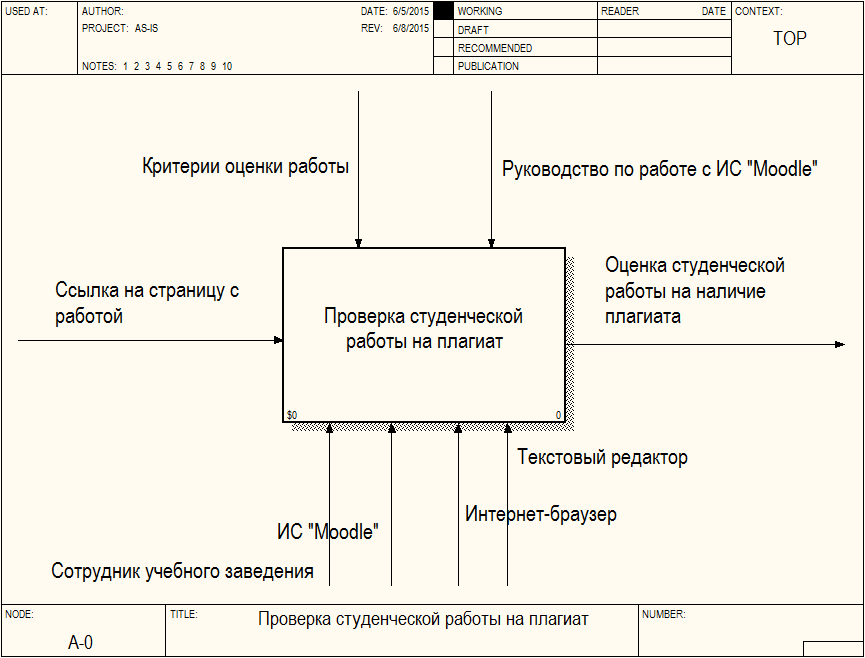
\includegraphics[width=\linewidth]{as_is_context.png}
				  \caption{Контекстная модель процесса до автоматизации}\label{img:as_is_context}
				\endminipage\hfill
				\minipage{0.49\textwidth}
				  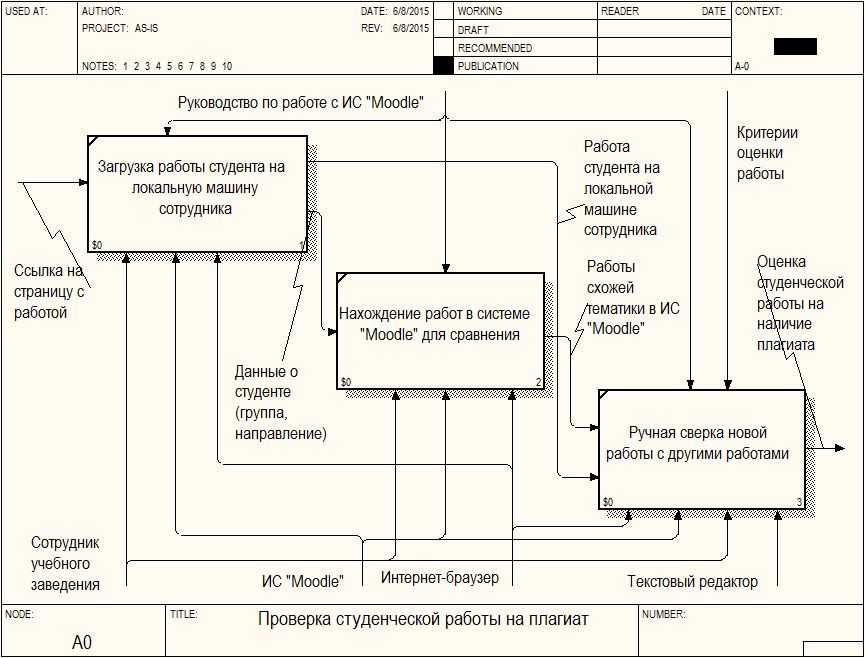
\includegraphics[width=\linewidth]{as_is_decomposition.png}
				  \caption{Декомпозиция контекстной модели}\label{img:as_is_decomposition}
				\endminipage\hfill				
			\end{figure}

			Наиболее трудозатратной операцией в процессе проверки на плагиат для сотрудника является ручная проверка работы на наличие заимствований. В качестве базы для сравнения используются работы всех студентов схожей тематики.			

			На вход в процесс поступает ссылка на документ в системе дистанцтионного обучения, который требуется проверить. Результатом выполнения процесса является оценка работы, исходя из результатов проверки.

		\subsubsection{Модель бизнес-процессов обработки информации («TO--BE»)}

			После анализ функциональной модели «AS--IS» была спроектирована модель «TO--BE», на которой отображается новая модель процесса проверки на плагиат, в которой сотруднику необходимо только принять решение на основе полученных результатов от ИС (степень совпадения и наиболее похожая работа), или запустить проверку, если она ещё не осуществлялась.

			На рисунках \ref{img:to_be_context} и \ref{img:to_be_decomposition} представлены контекстная диаграмма процесса после автоматизации и декомпозиция контекстной диаграммы 1-ого уровня соответственно.
			
			\begin{figure}[h]
				\minipage{0.49\textwidth}
				  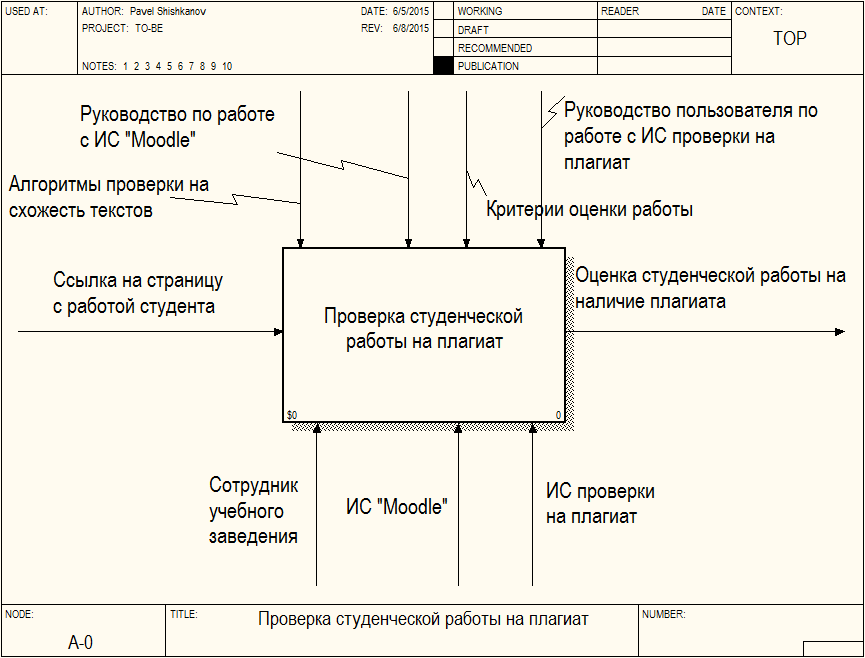
\includegraphics[width=\linewidth]{to_be_context.png}
				  \caption{Контекстная модель процесса после автоматизации}\label{img:to_be_context}
				\endminipage\hfill
				\minipage{0.49\textwidth}
				  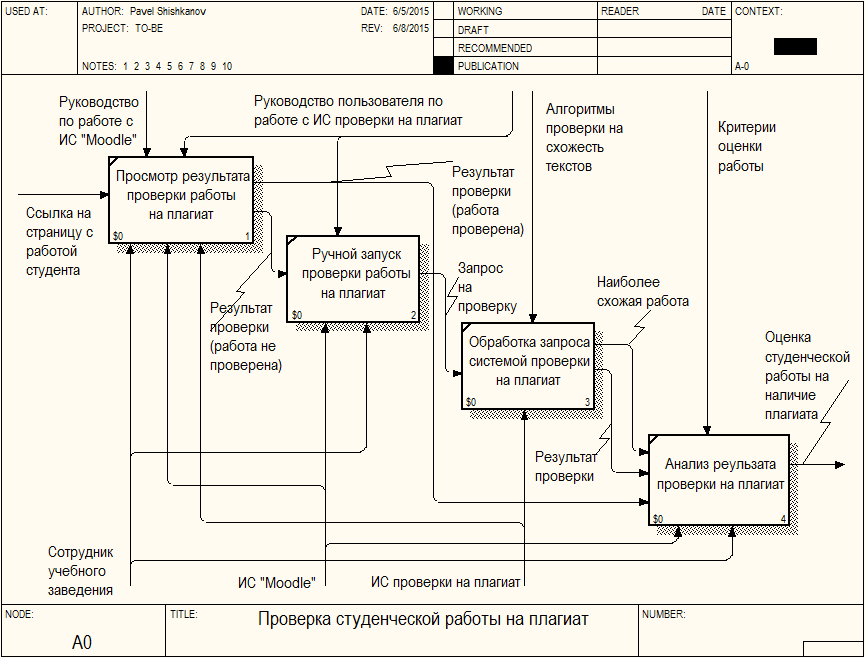
\includegraphics[width=\linewidth]{to_be_decomposition.png}
				  \caption{Декомпозиция контекстной модели}\label{img:to_be_decomposition}
				\endminipage\hfill				
			\end{figure}
